% Generated by tools/paper/render.py from main_text.py; edit the source there, not this file.
\documentclass[numsec,webpdf,modern,large]{oup-authoring-template}
\usepackage{booktabs}
\usetikzlibrary{plotmarks}
\begin{document}
\journaltitle{Bioinformatics}
\DOI{DOI added during production}
\copyrightyear{2026}
\pubyear{2026}
\access{Published: Date added during production}
\appnotes{Original Paper}
\firstpage{1}
\title[sporos]{sporos: one hardware-aware library to seed them all, from minimizers to maximal exact matches}
\author[1,$\ast$]{Konstantinos Kyriakidis}
\author[1,$\ast$]{Benedict Paten}
\address[1]{\orgname{UC Santa Cruz Genomics Institute}, \orgaddress{\state{Santa Cruz, CA}, \country{USA}}}
\corresp[$\ast$]{Corresponding authors. \href{mailto:kkyriaki@ucsc.edu}{kkyriaki@ucsc.edu}, \href{mailto:bpaten@ucsc.edu}{bpaten@ucsc.edu}}
\received{Date}{0}{Year}
\revised{Date}{0}{Year}
\accepted{Date}{0}{Year}
% Generated by tools/paper/render.py from main_text.py; edit the source there, not this file.
\abstract{\textbf{Motivation:} Read mappers, whole-genome aligners and pangenome tools all begin with seeds, short exact matches between a query and a reference. Each kind of seed is computed by its own tool: sampled k-mers such as minimizers and syncmers inside read mappers, maximal exact and unique matches (MEMs and MUMs) between genomes by MUMmer and copMEM2, super-maximal exact matches (SMEMs) of reads by BWA and its successors, and the recent frequency-capped MEMs and f-SMEMs by one or two tools each. Seeding takes a large share of read mapping: up to 60\% of BWA-MEM's time on short reads.\\
\textbf{Results:} We present sporos, a library that computes all of these seeds exactly, with one set of definitions and one interface. Its main algorithmic contribution counts the copies of a MEM's string from the MEMs themselves: a string occurs in the reference once for every MEM whose query interval contains its own, so frequency-capped MEMs need no index of the genomes beyond the one that finds the MEMs. On one Intel Skylake-X processor, sporos computed minimizers and syncmers 1.8--2.3 times faster than simd-minimizers on one core, looked seeds up 3.9 times faster than minimap2, found MEMs between two human chromosomes 1 2.0--2.4 times faster than copMEM2 and MUMs up to 43 times faster than MUMmer4 with identical output, frequency-capped MEMs 121--176 times faster than Mumemto, and SMEMs of short reads 4.8 times faster than minibwa.\\
\textbf{Availability and implementation:} sporos is free software under the MIT license, written in Mojo with C, Python and command-line interfaces, at \url{https://github.com/kokyriakidis/sporos}.}

\keywords{seeding, minimizers, syncmers, maximal exact matches, MUMs, SMEMs, FM-index, SIMD}
\maketitle
% Generated by tools/paper/render.py from main_text.py; edit the source there, not this file.
\section{Introduction}

Most analyses that compare DNA sequences begin by finding seeds, exact matches that indicate where a query and a reference may align. Read mappers chain seeds before alignment \citep{Li2013,Li2018}, whole-genome aligners anchor on matches unique to both genomes \citep{Delcher1999,Marcais2018}, and pangenome tools summarize shared sequence through matches common to many genomes \citep{Shivakumar2025}. Two families of seeds are in wide use. \emph{Sampled k-mers} retain a content-dependent subset of k-mers, so that copies of a region retain the same ones: minimizers, the k-mer of smallest hash in each window of w consecutive k-mers \citep{Schleimer2003,Roberts2004}, and syncmers, k-mers whose smallest s-mer lies at a fixed offset \citep{Edgar2021}. \emph{Maximal exact matches} (MEMs) extend until the sequences differ; maximal unique matches (MUMs) anchor whole-genome alignment \citep{Delcher1999}, and super-maximal exact matches (SMEMs), the MEMs of a read not contained in a longer one, seed BWA-MEM \citep{Li2012,Li2013}.

Seeding is a substantial cost. On short reads, single-threaded BWA-MEM spends 40--60\% of its time finding SMEMs and locating their occurrences \citep{Vasimuddin2019}, and dedicated hardware has been proposed to accelerate this step \citep{Subramaniyan2021}. The inputs keep growing, from complete telomere-to-telomere assemblies \citep{Nurk2022} to pangenomes of dozens of individuals \citep{Liao2023}, while the throughput of a processor core grows mainly through wider vector units and greater memory-level parallelism.

Each kind of seed is computed by a different tool on a different data structure. Minimizers are computed within read mappers such as minimap2 \citep{Li2018}, syncmers and strobemers within strobealign \citep{Sahlin2021,Sahlin2022}, and simd-minimizers computes random minimizers with SIMD instructions \citep{GrootKoerkamp2025simd}. MEMs and MUMs between genomes are found with suffix trees and suffix arrays in MUMmer \citep{Kurtz2004,Marcais2018}, with sparse suffix arrays \citep{Khan2009,Vyverman2013} and with hash tables of sampled k-mers in E-MEM and copMEM \citep{Khiste2015,Grabowski2019,Grabowski2023}. SMEMs are found with FM-indexes \citep{Ferragina2000} in BWA \citep{Li2013}, bwa-mem2 \citep{Vasimuddin2019}, ropebwt3 \citep{Li2024} and minibwa \citep{Li2026}. Newer seed types are supported by few tools. Mumemto relaxes multi-MUMs to matches that occur at most a given number of times, using the suffix array, LCP array and document array of the whole collection \citep{Shivakumar2025}. f-SMEMs, the maximal query intervals that occur at least f times, were introduced as k-MEMs \citep{Tatarnikov2022} and f-MEMs \citep{Gagie2026}, and ropebwt3 and minibwa compute them for read sets \citep{Li2024,Li2026}. Most of these tools parallelize across query sequences and process each sequence on one core, as a program built on a library would. We therefore compare the tools primarily on a single core, and also report ten threads, which matter most when a single long query, such as a chromosome, cannot be divided across sequences.

Here we present sporos, a library that computes all of these seeds exactly: minimizers and syncmers, a seed index for lookups, MEMs, MUMs and frequency-capped MEMs between genomes, and SMEMs and f-SMEMs of reads. It reproduces the definitions and output formats of the established tools, and on a single core it was faster than each of them. Our contributions are:

\begin{enumerate}
  \item \textbf{Frequency-capped MEMs without a collection index} (Section 3.4). The occurrences of a MEM's string in the reference correspond one to one to the MEMs whose query interval contains it (Lemma 1), so a sweep that retains the N largest interval ends counts occurrences up to a cap N.
  \item \textbf{Duplicate-free MEM enumeration} (Section 3.3). With the sparse sampling of copMEM \citep{Grabowski2019}, each MEM is reported by exactly one anchor, and anchor probes stream through a prefetching pipeline.
  \item \textbf{SMEM search with direct extension of unique matches} (Section 3.5). A match that occurs once is located and extended by comparing 32 bases at a time against the reference, and 16 reads are searched in interleaved fashion so that their memory accesses overlap.
  \item \textbf{Vectorized k-mer sampling} (Section 3.2). Minimizers and syncmers are computed on 8 or 16 SIMD lanes with exact leftmost tie-breaking and returned in sequence order from any number of threads; a seed index answers batched lookups through one prefetching pipeline.
  \item \textbf{A tested library} (Fig.~\ref{fig:overview}). One implementation per seed type serves the Mojo, C, Python and command-line interfaces; outputs equal those of MUMmer4 and copMEM2, and those of BWA except at ambiguous reference bases, and every kernel is tested against a brute-force oracle.
\end{enumerate}

On a single core of an Intel Skylake-X processor, sporos was faster than every other tool for every seed type we measured (Fig.~\ref{fig:speedups}), from 1.8 times faster than simd-minimizers for minimizers to 176 times faster than Mumemto for frequency-capped MEMs.

% Generated by tools/paper/render.py from main_text.py; edit the source there, not this file.
\section{Definitions}

Sequences are strings over \(\{A, C, G, T\}\); any other symbol, such as N, matches nothing, so no k-mer or match spans it. The reference \(R\) may contain several sequences, and matches do not cross sequence boundaries. \(S[i..j)\) denotes the substring of \(S\) from position \(i\) to \(j - 1\), and \(\overline{S}\) its reverse complement.

\textbf{Sampled k-mers.} For a hash \(h\) on k-mers, the (w, k)-minimizer of a window of w consecutive k-mers is its k-mer of minimum hash, with ties broken towards the leftmost; the minimizers of a sequence are those of all its windows, each reported once \citep{Roberts2004}. Canonical minimizers use a hash that is invariant under reverse complementation. A k-mer is a \emph{closed syncmer} if its minimal s-mer starts at offset 0 or \(k - s\), and an \emph{open syncmer} with offset t if it starts at t \citep{Edgar2021}. For comparison with simd-minimizers we use its parameterization, in which a syncmer is defined by the length k of the ranked substrings and their number w, and spans \(k + w - 1\) bases \citep{GrootKoerkamp2025simd}.

\textbf{Exact matches between genomes.} A \emph{MEM} of a query sequence \(Q\) and \(R\) is a triple \((r, q, \ell)\) with \(R[r..r+\ell) = Q[q..q+\ell)\) and \(\ell \ge L\) that cannot be extended to the left or right. It is a \emph{MUM} if its string occurs exactly once in \(R\) and once in \(Q\), and \emph{reference-unique} (MUMmer's \texttt{-mumreference}) if it occurs once in \(R\) \citep{Kurtz2004}. It is \emph{frequency-capped} at N if its string occurs at most N times in \(R\) or, in the strict form, at most N times in both \(R\) and \(Q\); a floor M additionally requires at least M occurrences in \(R\). N = 1 yields the MUMs. Reverse-strand matches are those of \(\overline{Q}\), with positions along \(\overline{Q}\), as in MUMmer.

\textbf{Exact matches of reads.} An interval \(Q[i..j)\) of a read \emph{occurs} if it or its reverse complement is a substring of \(R\). An \emph{SMEM} is an interval of length at least L that occurs and is not contained in a longer occurring interval \citep{Li2012}. An \emph{f-SMEM} replaces ``occurs'' by ``occurs at least f times'' \citep{Tatarnikov2022,Gagie2026}; f = 1 gives the SMEMs, and a cap N removes SMEMs that occur more than N times.

% Generated by tools/paper/render.py from main_text.py; edit the source there, not this file.
\section{Methods}

\subsection{Overview}

sporos is implemented in Mojo \citep{Mojo}, which compiles through MLIR \citep{Lattner2021} to native code and exposes SIMD vectors as first-class types. Input may be FASTA or FASTQ, plain, gzip- or BGZF-compressed, with BGZF blocks decompressed in parallel. Bases are stored as 2-bit codes, one per byte, with a fifth code for other symbols. Three engines compute the seeds (Fig.~\ref{fig:overview}); all are multithreaded with POSIX threads and exposed through a Mojo API, C and Python bindings and a command-line tool that writes MUMmer's MEM format and \texttt{bwa fastmap}'s SMEM format.

% Generated by tools/paper/render.py from main_text.py; edit the source there, not this file.
\begin{figure*}[t]
\centering
\resizebox{\textwidth}{!}{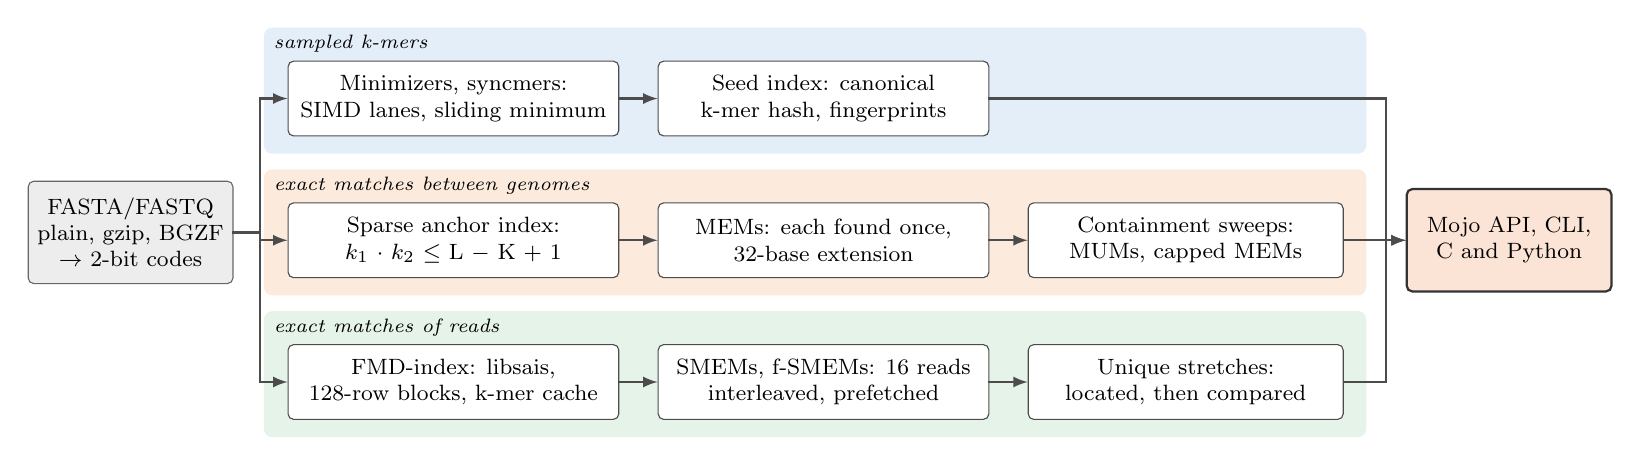
\begin{tikzpicture}
\fill[fill={rgb,255:red,227;green,238;blue,249}, rounded corners=3pt] (3.0,3.55) rectangle (17.0,5.15);\node[anchor=north west, font=\scriptsize\itshape, inner sep=2pt] at (3.05,5.130000000000001) {sampled k-mers};
\fill[fill={rgb,255:red,252;green,235;blue,221}, rounded corners=3pt] (3.0,1.75) rectangle (17.0,3.35);\node[anchor=north west, font=\scriptsize\itshape, inner sep=2pt] at (3.05,3.33) {exact matches between genomes};
\fill[fill={rgb,255:red,229;green,243;blue,232}, rounded corners=3pt] (3.0,-0.05) rectangle (17.0,1.55);\node[anchor=north west, font=\scriptsize\itshape, inner sep=2pt] at (3.05,1.53) {exact matches of reads};
\node[draw=black!60, fill={rgb,255:red,237;green,237;blue,237}, rounded corners=2pt, align=center, font=\footnotesize, inner sep=2pt, minimum width=2.6cm, minimum height=1.3cm, anchor=west] (input) at (0.0,2.55) {FASTA/FASTQ\\plain, gzip, BGZF\\$\to$ 2-bit codes};
\node[draw=black!70, fill={rgb,255:red,255;green,255;blue,255}, rounded corners=2pt, align=center, font=\footnotesize, inner sep=2pt, minimum width=4.2cm, minimum height=0.95cm, anchor=west] (window) at (3.3,4.25) {Minimizers, syncmers:\\SIMD lanes, sliding minimum};
\node[draw=black!70, fill={rgb,255:red,255;green,255;blue,255}, rounded corners=2pt, align=center, font=\footnotesize, inner sep=2pt, minimum width=4.2cm, minimum height=0.95cm, anchor=west] (seedindex) at (8.0,4.25) {Seed index: canonical\\k-mer hash, fingerprints};
\node[draw=black!70, fill={rgb,255:red,255;green,255;blue,255}, rounded corners=2pt, align=center, font=\footnotesize, inner sep=2pt, minimum width=4.2cm, minimum height=0.95cm, anchor=west] (anchors) at (3.3,2.45) {Sparse anchor index:\\$k_1$ $\cdot$ $k_2$ $\le$ L $-$ K + 1};
\node[draw=black!70, fill={rgb,255:red,255;green,255;blue,255}, rounded corners=2pt, align=center, font=\footnotesize, inner sep=2pt, minimum width=4.2cm, minimum height=0.95cm, anchor=west] (extend) at (8.0,2.45) {MEMs: each found once,\\32-base extension};
\node[draw=black!70, fill={rgb,255:red,255;green,255;blue,255}, rounded corners=2pt, align=center, font=\footnotesize, inner sep=2pt, minimum width=4.0cm, minimum height=0.95cm, anchor=west] (sweeps) at (12.7,2.45) {Containment sweeps:\\MUMs, capped MEMs};
\node[draw=black!70, fill={rgb,255:red,255;green,255;blue,255}, rounded corners=2pt, align=center, font=\footnotesize, inner sep=2pt, minimum width=4.2cm, minimum height=0.95cm, anchor=west] (fmd) at (3.3,0.65) {FMD-index: libsais,\\128-row blocks, k-mer cache};
\node[draw=black!70, fill={rgb,255:red,255;green,255;blue,255}, rounded corners=2pt, align=center, font=\footnotesize, inner sep=2pt, minimum width=4.2cm, minimum height=0.95cm, anchor=west] (search) at (8.0,0.65) {SMEMs, f-SMEMs: 16 reads\\interleaved, prefetched};
\node[draw=black!70, fill={rgb,255:red,255;green,255;blue,255}, rounded corners=2pt, align=center, font=\footnotesize, inner sep=2pt, minimum width=4.0cm, minimum height=0.95cm, anchor=west] (unique) at (12.7,0.65) {Unique stretches:\\located, then compared};
\node[draw=black!80, thick, fill={rgb,255:red,251;green,227;blue,214}, rounded corners=2pt, align=center, font=\footnotesize, inner sep=2pt, minimum width=2.6cm, minimum height=1.3cm, anchor=west] (api) at (17.5,2.45) {Mojo API, CLI,\\C and Python};
\draw[-latex, thick, black!70] (2.60,2.55) -- (2.95,2.55) -- (2.95,4.25) -- (3.30,4.25);
\draw[-latex, thick, black!70] (2.60,2.55) -- (2.95,2.55) -- (2.95,2.45) -- (3.30,2.45);
\draw[-latex, thick, black!70] (2.60,2.55) -- (2.95,2.55) -- (2.95,0.65) -- (3.30,0.65);
\draw[-latex, thick, black!70] (7.50,4.25) -- (8.00,4.25);
\draw[-latex, thick, black!70] (7.50,2.45) -- (8.00,2.45);
\draw[-latex, thick, black!70] (12.20,2.45) -- (12.70,2.45);
\draw[-latex, thick, black!70] (7.50,0.65) -- (8.00,0.65);
\draw[-latex, thick, black!70] (12.20,0.65) -- (12.70,0.65);
\draw[-latex, thick, black!70] (12.20,4.25) -- (17.25,4.25) -- (17.25,2.45) -- (17.50,2.45);
\draw[-latex, thick, black!70] (16.70,2.45) -- (17.50,2.45);
\draw[-latex, thick, black!70] (16.70,0.65) -- (17.25,0.65) -- (17.25,2.45) -- (17.50,2.45);
\end{tikzpicture}}
\caption{The sporos library. Input is parsed and coded once; three engines compute sampled k-mers and the seed index that looks them up (top), MEMs, MUMs and frequency-capped MEMs between genomes (middle), and SMEMs and f-SMEMs of reads (bottom), behind Mojo, command-line, C and Python interfaces.}\label{fig:overview}
\end{figure*}


\subsection{Minimizers and syncmers}

A single kernel computes minimizers and syncmers. As in simd-minimizers \citep{GrootKoerkamp2025simd}, the sequence is divided into contiguous chunks, one per SIMD lane: 16 with AVX-512 and 8 otherwise. Each lane rolls a 32-bit ntHash \citep{Mohamadi2016} with a rotation step of 7 instead of 1, which decorrelates the high bits of consecutive hashes; the canonical hash is the sum of the forward and reverse-complement hashes. Bases reach the lanes through a byte transpose, and each hash update is one byte-shuffle table lookup. Each k-mer is represented by a 32-bit key holding the high bits of its hash followed by its offset within a block of w consecutive k-mers, so that the sliding-window minimum, computed from prefix and suffix minima of these blocks with three \texttt{min} operations per k-mer (amortized), resolves ties to the leftmost k-mer exactly. k-mers containing other symbols receive a key above every valid one. Repeated minimizers are removed in the loop with one vector comparison, and surviving positions are collected every eight steps from a bit mask. Syncmers apply the same window minimum to s-mers.

For batches of short reads, each read occupies its own lane. For a long sequence on several threads, threads process short segments in order, and each copies its positions into the output once its predecessor has published where its positions end, yielding a single position list in sequence order without a merge.

\textbf{Seed index.} The seed index stores the minimizers, syncmers or all k-mers (k $\le$ 32) of a reference, keyed by canonical k-mer through an invertible mixing of its 2k bits. The high bits of the mixed key select a bucket and the remaining bits form a fingerprint; when bucket and fingerprint together hold 2k bits they identify the k-mer exactly, and otherwise candidates are verified against the reference. The table is built by a parallel radix sort. A batch of reads passes through one software pipeline that computes seeds, loads bucket bounds, compares fingerprints and prefetches subsequent probes across read boundaries. Seeds above an occurrence threshold, chosen as a quantile of the count distribution as in GraphAligner \citep{Rautiainen2020}, can be skipped.

\subsection{MEMs and MUMs}

Following copMEM \citep{Grabowski2019}, reference K-mers (K $\le$ 32) sampled every \(k_1\) positions are indexed and query K-mers sampled every \(k_2\) positions are looked up, with \(k_1\) and \(k_2\) coprime and \(k_1 k_2 \le L - K + 1\). By the Chinese remainder theorem, any \(k_1 k_2\) consecutive positions of a diagonal include one sampled in both sequences, so every MEM of length at least L contains an anchor. K, \(k_1\) and \(k_2\) are chosen for each L to minimize the estimated work, counting one unit per sampled reference position and three per probe. Each anchor hit is extended in both directions, 32 bases per comparison. Because the anchors of a MEM lie \(k_1 k_2\) apart along its diagonal, only the anchor whose leftward extension is shorter than \(k_1 k_2\) reports it, so each MEM is found exactly once without deduplication. The anchor table is built by a two-level radix sort with about four anchors per bucket, and probes are pipelined through hashing, bucket lookup, vectorized fingerprint comparison and prefetching of the reference text to be extended. MEMs are radix-sorted by query position.

By Lemma 1 (Section 3.4) with N = 1, a MEM is unique in the reference unless another MEM of the same query sequence contains it in query coordinates, and unique in the query unless another contains it in reference coordinates. MUMs therefore follow from two linear sweeps, one in query order and one after a parallel radix sort by reference position, each parallelized over blocks of MEMs.

\subsection{Frequency-capped MEMs}

\textbf{Lemma 1.} Let \(\mathcal{M}\) be the MEMs of length at least L of a query sequence \(Q\) against \(R\), and \(m = (r, q, \ell) \in \mathcal{M}\). The occurrences of \(Q[q..q+\ell)\) in \(R\) correspond one to one to the MEMs \((r', q', \ell') \in \mathcal{M}\) with \(q' \le q\) and \(q + \ell \le q' + \ell'\), and the occurrences of \(R[r..r+\ell)\) in \(Q\) to those with \(r' \le r\) and \(r + \ell \le r' + \ell'\).

\emph{Proof.} An occurrence of \(Q[q..q+\ell)\) at position \(p\) of \(R\) is a match on diagonal \(p - q\), which extends in both directions to a MEM whose query interval contains \([q, q+\ell)\); its length is at least \(\ell \ge L\), so it belongs to \(\mathcal{M}\). Distinct occurrences lie on distinct diagonals and give distinct MEMs. Conversely, a MEM \((r', q', \ell')\) whose query interval contains that of \(m\) holds an occurrence at \(p = r' + q - q'\). The second statement is symmetric. \(\square\)

Occurrence counts thus reduce to counting containing intervals among the MEMs. sporos processes the MEMs of each query sequence in order of start position, handling equal starts together, and maintains the N largest interval ends seen so far in a sorted buffer, discarding ends at or before the current start. The number of intervals containing an interval, capped at N, is the number of retained ends at or beyond its own end, found by binary search; with N = 1 this is the MUM test. Query-side counts use the same sweep in reference coordinates. The sweep is parallelized over blocks of MEMs, each block starting from the N largest ends of the preceding blocks, computed in a first pass. Each MEM costs \(O(\log N)\) for the search and at most \(O(N)\) for an insertion into the buffer. A floor M is handled by counting up to \(\max(N, M)\).

Mumemto instead traverses the suffix array, LCP array, BWT and document array of the whole collection, built by prefix-free parsing \citep{Shivakumar2025}. It defines matches over all genomes jointly and counts occurrences on both strands, so its output differs from that of sporos by definition (Section 4.5).

\subsection{SMEMs and f-SMEMs}

\textbf{Index.} sporos builds an FMD-index \citep{Li2012}: the Burrows--Wheeler transform \citep{BurrowsWheeler1994} of the maximal ACGT runs of the reference and their reverse complements, each terminated by a separator, so that the interval of a pattern is obtained together with that of its reverse complement and no match crosses a sequence end or a non-ACGT base. The suffix array is constructed in parallel with libsais \citep{libsais}. As in minibwa \citep{Li2026}, the transform is stored in 64-byte blocks of 128 rows, each holding four cumulative counts and 128 two-bit symbols; separators are stored as A and listed separately, with a flag on the few blocks that contain one. The ranks of all four bases are computed without branches using three population counts per word. The index also stores the 2-bit reference, 40-bit suffix-array samples and the interval of every k-mer for a k of up to 12, chosen by reference size, so that each search starts with one table lookup.

\textbf{Search.} SMEMs are found with the forward--backward algorithm \citep{Gagie2024} used by ropebwt3 and minibwa \citep{Li2024,Li2026}: from each start position, a backward search over L bases, a forward extension and a backward pass from the end of the match that determines the next start. When a match occurs only once, sporos stops traversing the index: it locates the occurrence, which the output requires anyway, and extends the match in both directions by comparing 32 bases at a time against the 2-bit reference. Sixteen reads are searched concurrently, their steps interleaved round-robin and each step prefetching the block its successor will access; occurrences of repeated SMEMs are located in batches in the same way. For f-SMEMs, each test for an empty interval becomes a test for fewer than f rows, and a cap N removes SMEMs with more than N occurrences. Threads process slices of reads.

The MEM engine yields the same SMEMs without an index: computed on both strands, the SMEMs are the MEM query intervals not contained in another, which suits single long queries such as whole chromosomes.

\subsection{Validation}

All kernels are tested in continuous integration against brute-force oracles that share no code with the library: minimizers and syncmers against exhaustive window scans, MEMs, MUMs and frequency-capped MEMs against enumeration of all pairs of start positions on repetitive sequences, and SMEMs and f-SMEMs against direct string search. The C and Python bindings are tested against the Mojo library.

% Generated by tools/paper/render.py from main_text.py; edit the source there, not this file.
\section{Results}

\subsection{Experimental setup}

Benchmarks ran on an Intel Core i9-7900X at 3.3~GHz (Skylake-X, AVX-512, ten cores) with turbo boost and hyper-threading disabled and 91~GB of memory, under Ubuntu Linux. sporos, simd-minimizers, minimap2, copMEM2 and strobealign were compiled for the native instruction set, minibwa with its default build, and MUMmer4, Mumemto, BWA and ropebwt3 were installed from Bioconda. The genome pairs were \emph{Escherichia coli} K-12 MG1655 and O157:H7 Sakai \citep{Blattner1997,Hayashi2001}, human (GRCh38 \citep{Schneider2017}) and chimpanzee (Clint \citep{Yoo2025}) chromosome 21, and GRCh38 and T2T-CHM13 \citep{Nurk2022} chromosome 1. Reads were simulated from GRCh38 chromosome 21: 1{,}000,000 of 150~bp and 4{,}000 of 10~kbp, each base replaced by a random base with probability 0.002 and half of the reads reverse-complemented. Unless stated otherwise, each command was run three times (once if it exceeded 60~s) after the machine became idle, and the best wall time is reported; MEM and SMEM tools wrote their output to files, except ropebwt3, whose output was discarded. Supplementary Section S1 lists versions and commands.

\subsection{Minimizers and syncmers}

On one thread, sporos computed minimizers and closed syncmers 1.8--2.3 times faster than simd-minimizers across all schemes on CHM13 chromosome 1 and on random DNA (Table~\ref{tab:seeds}; Supplementary Table S2); canonical (21, 11)-minimizers of chromosome 1 took 1.11~ns per base (0.90 Gbp/s). With 8 lanes, the vector width of simd-minimizers, sporos was 1.3--1.7 times faster on chromosome 1, and the 16-lane AVX-512 build was another 1.27--1.48 times faster, whereas simd-minimizers reported a slowdown with AVX-512 \citep{GrootKoerkamp2025simd}. minimap2's \texttt{mm\_sketch} was 15 times slower than sporos. On ten threads, sporos was between 1.1 times slower and 1.6 times faster than simd-minimizers; our harness for simd-minimizers only counts each thread's positions, whereas sporos returns one ordered list.

% Generated by tools/paper/render.py from main_text.py; edit the source there, not this file.
\begin{table*}[t]
\caption{Minimizers and closed syncmers of CHM13 chr1 (248~Mbp): ns per base, the best of 5 to 7 runs on one thread and of 3 on ten. Every tool reads its input already encoded (simd-minimizers packed at two bits per base, sporos at one byte per base, minimap2's mm\_sketch in ASCII) and writes positions to memory. sporos runs 16 lanes of 32 bits (AVX-512) or 8 (the width simd-minimizers uses, AVX2). mm\_sketch computes canonical minimizers only, of k at most 28 (the k = 31 rows run k = 28). Bold: fastest at each thread count.}\label{tab:seeds}
\centering\footnotesize
\setlength{\tabcolsep}{4pt}
\resizebox{\ifdim\width>\textwidth\textwidth\else\width\fi}{!}{\begin{tabular}{@{}llrrrrrrr@{}}
\toprule
 &  & \multicolumn{4}{c}{One thread} & \multicolumn{3}{c}{Ten threads} \\ \cmidrule(lr){3-6}\cmidrule(lr){7-9}
Scheme & k, w & sporos-16 & sporos-8 & simd-min. & mm\_sketch & sporos-16 & simd-min. & mm\_sketch \\
\midrule
Minimizers, forward & 21, 11 & \textbf{1.04} & 1.33 & 1.81 & -- & 0.259 & \textbf{0.192} & -- \\
Minimizers, canonical & 21, 11 & \textbf{1.02} & 1.44 & 2.17 & 17.1 & 0.268 & \textbf{0.206} & 1.97 \\
Closed syncmers, forward & 21, 11 & \textbf{1.14} & 1.45 & 2.00 & -- & \textbf{0.183} & 0.197 & -- \\
Closed syncmers, canonical & 21, 11 & \textbf{1.16} & 1.58 & 2.57 & -- & \textbf{0.180} & 0.248 & -- \\
Minimizers, forward & 31, 19 & \textbf{0.926} & 1.24 & 1.62 & -- & \textbf{0.125} & 0.156 & -- \\
Minimizers, canonical & 31, 19 & \textbf{0.923} & 1.34 & 1.91 & 15.3 & \textbf{0.138} & 0.189 & 1.92 \\
Closed syncmers, forward & 31, 19 & \textbf{0.992} & 1.31 & 1.85 & -- & \textbf{0.136} & 0.174 & -- \\
Closed syncmers, canonical & 31, 19 & \textbf{1.01} & 1.46 & 2.33 & -- & \textbf{0.135} & 0.225 & -- \\
\bottomrule
\end{tabular}}
\end{table*}


\subsection{Seed-index lookups}

Seeding 150~bp reads and looking up their minimizers, sporos processed 136~Mbp per second on one thread, 3.9 times the throughput of minimap2 (34.6~Mbp/s) for the same minimizers and occurrence cap, and 9.3 times that of strobealign for its randstrobes (Table~\ref{tab:lookups}). With one read per call, sporos remained 1.4 times faster than minimap2.

% Generated by tools/paper/render.py from main_text.py; edit the source there, not this file.
\begin{table}[t]
\caption{Seed-index lookups of 1 M simulated 150~bp reads against hg38 chr21 on one thread: throughput in Mbp of reads per second, the best of three runs, reads in memory, timing only the loop that seeds each read and copies out its hits; index build time on 1 and 8 threads. sporos and minimap2 index the same (w, k)-minimizers under different hashes and skip seeds with more than 20 hits; strobealign indexes randstrobes with its defaults for 150~bp reads and does more per seed (both orientations, partial-strobe lookups), so its rows are a reference point. minimap2's and strobealign's build times include reading the FASTA file.}\label{tab:lookups}
\centering\footnotesize
\setlength{\tabcolsep}{4pt}
\resizebox{\linewidth}{!}{\begin{tabular}{@{}lrrr@{}}
\toprule
Seeding & Mbp/s & Hits per read & Build (s), 1 / 8 threads \\
\midrule
sporos, batch (k = 19, w = 12) & \textbf{136} & 27.7 & 0.338 / 0.0645 \\
sporos, one read per call (k = 19, w = 12) & 47.0 & 27.7 &  \\
minimap2 (k = 19, w = 12) & 34.6 & 27.6 & 1.64 / 1.22 \\
sporos, batch (k = 21, w = 11) & \textbf{131} & 29.0 & 0.357 / 0.0675 \\
sporos, one read per call (k = 21, w = 11) & 46.4 & 29.0 &  \\
minimap2 (k = 21, w = 11) & 32.6 & 29.1 & 1.66 / 1.25 \\
strobealign, one hit per seed & 14.7 & 51.0 & 1.77 / 1.33 \\
strobealign, every position & 13.1 & 97.2 &  \\
\bottomrule
\end{tabular}}
\end{table}


\subsection{MEMs and MUMs}

On one thread, sporos found all MEMs of the three genome pairs 2.0--16 times faster than copMEM2, and 2.0--2.4 times faster on the chromosome 1 pair (Table~\ref{tab:mems}; Supplementary Table S3). As neither copMEM2 nor MUMmer4 divides a single query sequence among threads, sporos was 9.7--12 times faster than copMEM2 on ten threads, finding the 65.6 million MEMs of at least 50~bp between the chromosomes 1 in 3.74~s. sporos was 4.2--43 times faster than MUMmer4 for MEMs, MUMs and reference-unique MEMs (Supplementary Table S4); the smallest margin was for MUMs of the chromosome 1 pair, for which sporos first enumerates all 65.6 million MEMs. All 60 output checks passed: the outputs of sporos equalled those of MUMmer4 and copMEM2, and its ten-thread outputs its one-thread outputs. Peak memory on chromosome 1 was at most 3.5~GB (Supplementary Table S5).

% Generated by tools/paper/render.py from main_text.py; edit the source there, not this file.
\begin{table*}[t]
\caption{MEMs and MUMs of at least 50~bp between whole chromosomes, forward strand: wall time in seconds, the best of three runs (one run past 60~s), output written to a file. copMEM2 is the faster of its default and \texttt{-mf} settings; it and MUMmer4 gain nothing from more threads on a single query sequence (Supplementary Section S1). Every sporos output equals MUMmer4's, and its MEMs equal copMEM2's. Bold: fastest at each thread count.}\label{tab:mems}
\centering\footnotesize
\setlength{\tabcolsep}{4pt}
\resizebox{\ifdim\width>\textwidth\textwidth\else\width\fi}{!}{\begin{tabular}{@{}lrrrrrrrr@{}}
\toprule
 & \multicolumn{5}{c}{MEMs (\texttt{-maxmatch})} & \multicolumn{3}{c}{MUMs (\texttt{-mum})} \\ \cmidrule(lr){2-6}\cmidrule(lr){7-9}
Pair & sporos, 1 thr. & sporos, 10 thr. & copMEM2, 1 thr. & copMEM2, 10 thr. & MUMmer4 & sporos, 1 thr. & sporos, 10 thr. & MUMmer4 \\
\midrule
E. coli (4.6 / 5.5~Mbp) & \textbf{0.09} & \textbf{0.05} & 0.89 & 0.89 & 1.97 & \textbf{0.09} & 0.05 & 1.71 \\
Human / chimpanzee chr21 (47 / 33~Mbp) & \textbf{0.72} & \textbf{0.23} & 1.95 & 1.95 & 17.5 & \textbf{0.73} & 0.25 & 14.6 \\
hg38 / CHM13 chr1 (249 / 248~Mbp) & \textbf{19.5} & \textbf{3.74} & 46.3 & 46.4 & 159 & \textbf{21.0} & 3.97 & 87.5 \\
\bottomrule
\end{tabular}}
\end{table*}


\subsection{Frequency-capped MEMs}

sporos computed frequency-capped MEMs 121--176 times faster than Mumemto on one thread, using 8--18\% of its memory (Table~\ref{tab:capped}). The definitions differ, so the comparison is between the closest settings: Mumemto treats both genomes as one collection, counts occurrences on both strands and considers a match maximal if its occurrences cannot all be extended together, whereas sporos reports MUMmer-style position pairs of the query against the reference and counts occurrences in the reference as given. On the \emph{E. coli} pair, sporos reported 89--99\% of the forward-strand position pairs of Mumemto, and Mumemto 97--100\% of those of sporos. On chromosome 21 these shares were 32--93\% and 77--93\%, which we attribute to the two notions of maximality: in repeats, two copies of a string that is maximal across the collection can extend further as a pair, and sporos then reports the longer match.

% Generated by tools/paper/render.py from main_text.py; edit the source there, not this file.
\begin{table*}[t]
\caption{Frequency-capped MEMs of at least 50~bp on both strands: wall time in seconds and peak memory in MB. Mumemto (one thread) finds the multi-MEMs of the two genomes as one collection, capped per genome (\texttt{-k 2 -f N}) or in total (\texttt{-k 2 -f 0 -F N}); sporos finds the MEMs of the query against the reference whose string occurs at most N times in the reference (\texttt{-maxmatch -{}-max-occ N}, for the total cap) or in the reference and the query (\texttt{-mum -{}-max-occ N}, per genome). The definitions differ (Section 4.5): the last column gives the share of Mumemto's forward-strand position pairs that sporos also reports, and of sporos's that Mumemto reports.}\label{tab:capped}
\centering\footnotesize
\setlength{\tabcolsep}{4pt}
\resizebox{\ifdim\width>\textwidth\textwidth\else\width\fi}{!}{\begin{tabular}{@{}lrrrrrrr@{}}
\toprule
Pair and cap & sporos, 1 thr. & sporos, 10 thr. & Mumemto & Speedup & sporos MB & Mumemto MB & Shared (\%) \\
\midrule
E. coli, at most 3 per genome & \textbf{0.11} & 0.06 & 13.3 & 121 & 61 & 348 & 97 / 99 \\
E. coli, at most 10 per genome & \textbf{0.11} & 0.06 & 13.3 & 121 & 61 & 348 & 89 / 100 \\
E. coli, at most 3 in total & \textbf{0.10} & 0.05 & 13.3 & 133 & 61 & 348 & 99 / 97 \\
E. coli, at most 10 in total & \textbf{0.10} & 0.06 & 13.3 & 133 & 61 & 348 & 94 / 99 \\
chr21, at most 3 per genome & \textbf{1.02} & 0.31 & 169 & 166 & 257 & 3{,}130 & 77 / 93 \\
chr21, at most 10 per genome & \textbf{1.05} & 0.33 & 170 & 162 & 257 & 3{,}130 & 32 / 88 \\
chr21, at most 3 in total & \textbf{0.96} & 0.28 & 169 & 176 & 257 & 3{,}130 & 93 / 83 \\
chr21, at most 10 in total & \textbf{0.98} & 0.28 & 170 & 174 & 257 & 3{,}130 & 54 / 77 \\
\bottomrule
\end{tabular}}
\end{table*}


\subsection{SMEMs and f-SMEMs}

On one thread, sporos found the SMEMs of 150~bp reads 4.8 times faster than minibwa, 15 times faster than \texttt{bwa fastmap} and 51 times faster than ropebwt3 without position output, and those of 10~kbp reads 5.7, 17 and 65 times faster (Table~\ref{tab:smems}). For f-SMEMs, sporos was 2.3 times faster than minibwa at f = 2 and 2.3 times at f = 5, and 32 and 29 times faster than ropebwt3. Requiring two occurrences slowed the search 4.2 times relative to SMEMs, since a match that occurs once no longer ends it. sporos and \texttt{bwa fastmap} differed in 20 of 1.22 million SMEMs of the short reads; all 14 reported only by BWA pass through an N of the reference, which BWA replaces with random bases (Supplementary Section S3). Ten threads gave the same SMEMs as one.

% Generated by tools/paper/render.py from main_text.py; edit the source there, not this file.
\begin{table*}[t]
\caption{SMEMs (f = 1) and f-SMEMs of at least 19~bp of simulated reads against hg38 chr21, both strands: wall time in seconds, the best of three runs, the index loaded from disk. sporos, minibwa and bwa fastmap list the positions of SMEMs with at most 20 hits; ropebwt3 is run without positions, its default, which favours it. minibwa and bwa fastmap are single-threaded; bwa computes no f-SMEMs. Bold: fastest at each thread count.}\label{tab:smems}
\centering\footnotesize
\setlength{\tabcolsep}{4pt}
\resizebox{\ifdim\width>\textwidth\textwidth\else\width\fi}{!}{\begin{tabular}{@{}lrrrrrr@{}}
\toprule
 & \multicolumn{4}{c}{One thread} & \multicolumn{2}{c}{Ten threads} \\ \cmidrule(lr){2-5}\cmidrule(lr){6-7}
Reads & sporos & minibwa & bwa & ropebwt3 & sporos & ropebwt3 \\
\midrule
1 M reads of 150~bp, SMEMs & \textbf{1.85} & 8.95 & 27.5 & 93.5 & \textbf{0.40} & 9.64 \\
1 M reads of 150~bp, f = 2 & \textbf{7.79} & 17.6 & -- & 246 & \textbf{1.09} & 24.9 \\
1 M reads of 150~bp, f = 5 & \textbf{7.51} & 17.5 & -- & 216 & \textbf{1.10} & 21.9 \\
4{,}000 reads of 10~kbp, SMEMs & \textbf{0.37} & 2.11 & 6.37 & 24.1 & \textbf{0.14} & 2.49 \\
4{,}000 reads of 10~kbp, f = 2 & \textbf{2.45} & 5.36 & -- & 73.8 & \textbf{0.41} & 7.51 \\
4{,}000 reads of 10~kbp, f = 5 & \textbf{2.41} & 5.40 & -- & 65.0 & \textbf{0.39} & 6.64 \\
\bottomrule
\end{tabular}}
\end{table*}


% Generated by tools/paper/render.py from main_text.py; edit the source there, not this file.
\begin{figure}[t]
\centering
\resizebox{\linewidth}{!}{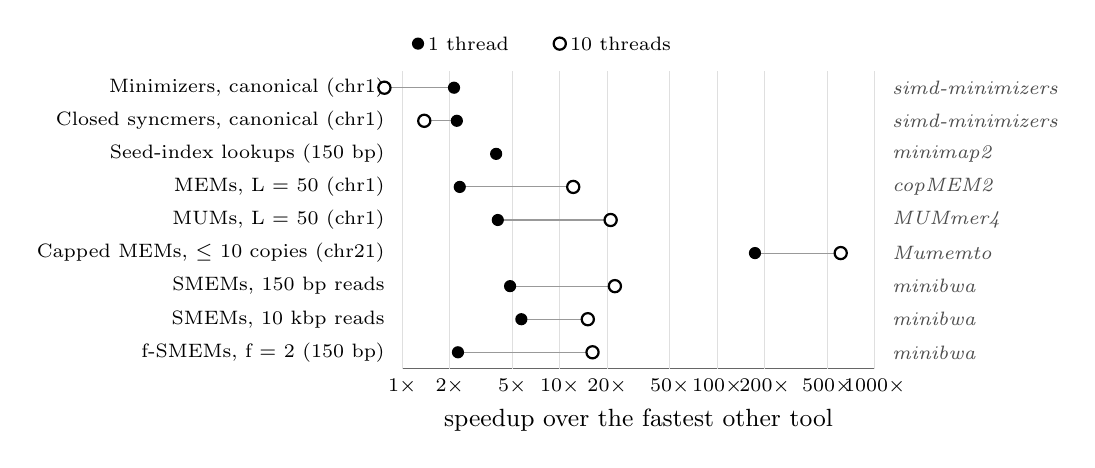
\begin{tikzpicture}
\draw[black!60] (0,0) -- (6.0,0);
\draw[gray!25] (0.000,0) -- (0.000,3.780);\node[below, font=\scriptsize] at (0.000,0) {1$\times$};
\draw[gray!25] (0.602,0) -- (0.602,3.780);\node[below, font=\scriptsize] at (0.602,0) {2$\times$};
\draw[gray!25] (1.398,0) -- (1.398,3.780);\node[below, font=\scriptsize] at (1.398,0) {5$\times$};
\draw[gray!25] (2.000,0) -- (2.000,3.780);\node[below, font=\scriptsize] at (2.000,0) {10$\times$};
\draw[gray!25] (2.602,0) -- (2.602,3.780);\node[below, font=\scriptsize] at (2.602,0) {20$\times$};
\draw[gray!25] (3.398,0) -- (3.398,3.780);\node[below, font=\scriptsize] at (3.398,0) {50$\times$};
\draw[gray!25] (4.000,0) -- (4.000,3.780);\node[below, font=\scriptsize] at (4.000,0) {100$\times$};
\draw[gray!25] (4.602,0) -- (4.602,3.780);\node[below, font=\scriptsize] at (4.602,0) {200$\times$};
\draw[gray!25] (5.398,0) -- (5.398,3.780);\node[below, font=\scriptsize] at (5.398,0) {500$\times$};
\draw[gray!25] (6.000,0) -- (6.000,3.780);\node[below, font=\scriptsize] at (6.000,0) {1000$\times$};
\node[font=\small] at (3.00,-0.65) {speedup over the fastest other tool};
\node[anchor=east, font=\scriptsize] at (-0.10,3.570) {Minimizers, canonical (chr1)};
\node[anchor=west, font=\scriptsize\itshape, black!70] at (6.10,3.570) {simd-minimizers};
\draw[black!40] (-0.227,3.570) -- (0.657,3.570);
\fill[black] (0.657,3.570) circle (2.2pt);
\draw[black, fill=white, thick] (-0.227,3.570) circle (2.2pt);
\node[anchor=east, font=\scriptsize] at (-0.10,3.150) {Closed syncmers, canonical (chr1)};
\node[anchor=west, font=\scriptsize\itshape, black!70] at (6.10,3.150) {simd-minimizers};
\draw[black!40] (0.279,3.150) -- (0.693,3.150);
\fill[black] (0.693,3.150) circle (2.2pt);
\draw[black, fill=white, thick] (0.279,3.150) circle (2.2pt);
\node[anchor=east, font=\scriptsize] at (-0.10,2.730) {Seed-index lookups (150 bp)};
\node[anchor=west, font=\scriptsize\itshape, black!70] at (6.10,2.730) {minimap2};
\fill[black] (1.192,2.730) circle (2.2pt);
\node[anchor=east, font=\scriptsize] at (-0.10,2.310) {MEMs, L = 50 (chr1)};
\node[anchor=west, font=\scriptsize\itshape, black!70] at (6.10,2.310) {copMEM2};
\draw[black!40] (0.730,2.310) -- (2.171,2.310);
\fill[black] (0.730,2.310) circle (2.2pt);
\draw[black, fill=white, thick] (2.171,2.310) circle (2.2pt);
\node[anchor=east, font=\scriptsize] at (-0.10,1.890) {MUMs, L = 50 (chr1)};
\node[anchor=west, font=\scriptsize\itshape, black!70] at (6.10,1.890) {MUMmer4};
\draw[black!40] (1.213,1.890) -- (2.646,1.890);
\fill[black] (1.213,1.890) circle (2.2pt);
\draw[black, fill=white, thick] (2.646,1.890) circle (2.2pt);
\node[anchor=east, font=\scriptsize] at (-0.10,1.470) {Capped MEMs, $\le$ 10 copies (chr21)};
\node[anchor=west, font=\scriptsize\itshape, black!70] at (6.10,1.470) {Mumemto};
\draw[black!40] (4.479,1.470) -- (5.568,1.470);
\fill[black] (4.479,1.470) circle (2.2pt);
\draw[black, fill=white, thick] (5.568,1.470) circle (2.2pt);
\node[anchor=east, font=\scriptsize] at (-0.10,1.050) {SMEMs, 150 bp reads};
\node[anchor=west, font=\scriptsize\itshape, black!70] at (6.10,1.050) {minibwa};
\draw[black!40] (1.369,1.050) -- (2.700,1.050);
\fill[black] (1.369,1.050) circle (2.2pt);
\draw[black, fill=white, thick] (2.700,1.050) circle (2.2pt);
\node[anchor=east, font=\scriptsize] at (-0.10,0.630) {SMEMs, 10 kbp reads};
\node[anchor=west, font=\scriptsize\itshape, black!70] at (6.10,0.630) {minibwa};
\draw[black!40] (1.512,0.630) -- (2.356,0.630);
\fill[black] (1.512,0.630) circle (2.2pt);
\draw[black, fill=white, thick] (2.356,0.630) circle (2.2pt);
\node[anchor=east, font=\scriptsize] at (-0.10,0.210) {f-SMEMs, f = 2 (150 bp)};
\node[anchor=west, font=\scriptsize\itshape, black!70] at (6.10,0.210) {minibwa};
\draw[black!40] (0.707,0.210) -- (2.416,0.210);
\fill[black] (0.707,0.210) circle (2.2pt);
\draw[black, fill=white, thick] (2.416,0.210) circle (2.2pt);
\fill[black] (0.2,4.130) circle (2.2pt) node[right, font=\scriptsize] {1 thread};\draw[black, fill=white, thick] (2.0,4.130) circle (2.2pt) node[right, font=\scriptsize] {10 threads};
\end{tikzpicture}}
\caption{Speedup of sporos over the fastest other tool for each task, on one thread (filled) and ten (hollow), each tool at its best on that many threads; the other tool is named on the right (Tables 1 to 5). copMEM2, MUMmer4, minibwa, bwa fastmap and Mumemto use one thread; the seed-lookup harnesses run one.}\label{fig:speedups}
\end{figure}


% Generated by tools/paper/render.py from main_text.py; edit the source there, not this file.
\section{Discussion}

sporos computes the seeds used by read mappers, genome aligners and pangenome tools, following the established definitions, and on a single core it was faster than each tool it can replace. Its frequency-capped MEMs show that how often each match's string occurs can be derived from the set of matches itself: counting containing intervals replaces an index of the genomes and reduces capped matching between two chromosomes to about a second.

A single library also avoids converting between tools. A pipeline loads a reference once and requests MEMs, MUMs or SMEMs from Mojo, C or Python, with one coordinate system and one set of occurrence limits, and the command-line tool writes the MUMmer and \texttt{bwa fastmap} formats that existing scripts expect.

\textbf{Limitations.} All measurements were taken on one x86-64 processor; the 8-lane rows of Table~\ref{tab:seeds} indicate performance at AVX2 width, but other processors, including ARM, were not benchmarked. Mumemto was compared on pairs of genomes rather than the large collections it targets, and its definitions differ from those of sporos. Positions are 32-bit, limiting each sequence and the concatenated reference to fewer than \(2^{32}\) bases, and FM-index construction needs about ten bytes of memory per reference base. On ten threads sporos was slower than simd-minimizers for one of the eight schemes.

% Generated by tools/paper/render.py from main_text.py; edit the source there, not this file.
\section*{Author contributions}
Konstantinos Kyriakidis (Conceptualization [lead], Methodology [lead], Software [lead], Validation [lead], Formal analysis [lead], Investigation [lead], Data curation [lead], Visualization [lead], Writing---original draft [lead]), Benedict Paten (Supervision [lead], Writing---review \& editing [equal]).

\section*{Supplementary data}
Supplementary data are available at \emph{Bioinformatics} online.

\section*{Conflict of interest}
None declared.

\section*{Funding}
This work received no specific funding.

\section*{Data availability}
The software and the benchmark scripts are available at \url{https://github.com/kokyriakidis/sporos}; \texttt{benchmarks/competitors/} sets up every tool at a pinned version, downloads the genomes, simulates the reads and runs each benchmark, and its \texttt{results/} directory holds the raw measurements behind every table.

\bibliographystyle{oup-abbrvnat}
\bibliography{references}
\end{document}
